
\begin{savequote}[50mm]
There is much pleasure to be gained from useless knowledge.
%\footnotemark[1]
\qauthor{Bertrand Russell}
\end{savequote}

\chapter{LTS-HLL-type schemes}
\label{cha:LTS-HLL}

%\footnotetext[1]{In \textit{In Praise of Idleness and Other Essays} (1935).}
%\setcounter{footnote}{1}

This chapter presents the main results of this thesis. These results have been already described in \ref{cha1:sec:goals}~\textit{Goals and thesis outline}, but we repeat them to give the structure of the chapter:
\begin{itemize}
\item In \cref{sec:LTS-HLL(C)} we develop the framework of the LTS-HLL-type schemes, and we develop LTS-HLL(C) schemes.

\item In \cref{sec:EV-ME} we investigate entropy stability of the LTS methods by using the modified equation analysis.

\item In \cref{sec:PP} we investigate monotonicity and positivity preservation of the LTS methods. 
\end{itemize}

\section{Constructing the LTS-HLL and LTS-HLLC schemes}
\label{sec:LTS-HLL(C)}

The HLL~(Harten--Lax--van Leer) solver was proposed by Harten et al.~\cite{har83a} as an example of a very simple and inexpensive approximate Riemann solver for systems of hyperbolic conservation laws. In the original paper, the HLL scheme assumes a two-wave structure of the solution and constructs the approximate Riemann solver by using estimates of the velocities for the slowest and fastest waves. The choice of these estimates plays a decisive role for the properties of the scheme. Namely, by an appropriate choice of the wave velocity estimates it is possible to tune the amount of numerical diffusion, recover some existing numerical methods and achieve an entropy stable and a positivity preserving scheme. 

The choice of wave velocity estimates has been studied for instance by Davis~\cite{dav88}, Einfeldt and co-workers~\cite{ein88,ein91}, Toro et al.~\cite{tor94}, Batten et al.~\cite{bat97}, Bouchut~\cite{bou04}, Pelanti~\cite{pel01} and LeVeque and Pelanti~\cite{lev01}. In particular, the choice of wave velocities according to Einfeldt~\cite{ein88} became very popular because it yields an entropy stable and a positivity preserving scheme, known as the HLLE scheme. However, simplicity of the HLL scheme is owing to the fact that it is an \textit{incomplete} Riemann solver. Namely, by assuming a two-wave structure of the solution, the HLL scheme imposes a single intermediate state across the Riemann fan. Because of this, the HLL scheme may poorly resolve certain waves in systems where solution structure consists of more than two waves. Einfeldt~\cite{ein88}, Linde~\cite{lin02} and Park~\cite{par03} introduced modifications of the HLL scheme in which the resolution of intermediate waves is improved. For the Euler equations, Toro et al.~\cite{tor94} proposed the HLLC~(HLL--Contact) solver in which the contact discontinuity is reconstructed by assuming a three-wave structure of the solution.

As stated above, the original HLL scheme assumes a two-wave structure of the solution and it was originally intended as a solver for systems of equations. Later developments of the HLL scheme continued to work along these lines, and the same applies to the HLLC scheme which was designed as a solver for the Euler equations. We followed this same approach in our paper~\cite{jp2} where we used the HLL and HLLC schemes for the system of conservation laws as the starting point.

Herein, we adopt a slightly different approach and interpret the HLL scheme as a method for scalar conservation laws. We define the HLL-type schemes, a class of standard \textit{two-parameter} methods that also includes the one-parameter methods \eqref{eq:scalar-Q} and \eqref{eq:scalar-A} considered in \cref{cha:Background}. The new framework can be written in both numerical viscosity \eqref{eq:scalar-NV} and flux-difference splitting form \eqref{eq:scalar-FDS}. By introducing notion of \textit{waves}~\cite{lev02}, we can also write the new scheme in \textit{wave propagation} form, which will provide a new insight into the TVD condition. Further, by interpreting the HLL scheme as a scheme for a scalar conservation law we are able to rigorously study its convergence and entropy stability.

The extension to the LTS-HLL scheme is made as in the previous chapter, following the work of Lindqvist et al.~\cite{lin16}. We define a class of LTS two-parameter methods, which allows us to obtain LTS extensions of some standard one-parameter methods in a very simple way. Lastly, the extension to systems of equations is done as earlier by a classical field-by-field decomposition into characteristic variables.

A number of ideas that will be used in this section have been recognized and used by different authors, for instance Harten and Hyman~\cite{har83c}, LeVeque~\cite{lev92,lev02}, Bouchut~\cite{bou04}, Pelanti~\cite{pel01} and Einfeldt~\cite{ein88}. Our framework naturally incorporates these ideas as will be described in more detail below.

\subsection{Standard HLL scheme for scalar conservation laws}

Once again, we are interested in solving the scalar conservation law \eqref{eq:SCL}:
\begin{equation} \label{eq:SCL2}
u_t + f(u)_x = 0.
\end{equation}
In the previous chapter we solved \eqref{eq:SCL2} by using standard one-parameter methods written in the numerical viscosity \eqref{eq:scalar-NV} and flux-difference splitting \eqref{eq:scalar-FDS} form. Herein, our first goal is to establish the HLL scheme.

We start by retaining the basic assumption of HLL-type schemes and assume a two-wave structure of the solution. This leads to a simplest possible two-wave Riemann solver:
\begin{equation} \label{eq:scalar-RP-HLL}
\widetilde{u}_{j+1/2}(x/t) = \left\{ \begin{array}{lll}
	u_j		 \quad \quad & \text{if} \quad x < \SLj t, \\[0.25em]
	u_{j+1/2}^\text{HLL} & \text{if} \quad \SLj t < x < \SRj t, \\[0.25em]
	u_{j+1}       		 & \text{if} \quad x > \SRj t,\end{array} \right.
\end{equation}
where $ \SLj $ and $ \SRj $ are wave velocity estimates (that are to be determined later on), while $ u_{j+1/2}^\text{HLL} $ is the intermediate state such that the Riemann solver \eqref{eq:scalar-RP-HLL} is consistent with the integral form of the conservation law \eqref{eq:SCL2}:
\begin{equation} \label{eq:scalar-uHLL}
u_{j+1/2}^{\text{HLL}} = \frac{\SR u_{j+1} - \SL u_j + f_j - f_{j+1}}{\SR - \SL},
\end{equation}
where we suppressed the interface index on $ \SL $ and $ \SR $ because the interface index is given on the left-hand side. We refer to Toro~\cite[p.~319]{tor09} for step by step derivation of \eqref{eq:scalar-uHLL}. By using \eqref{eq:scalar-RP-HLL} in \eqref{eq:convex-update} we may write the HLL scheme in the conservation form \eqref{eq:scalar-CF} with the numerical flux function:
\begin{equation} \label{eq:scalar-FHLL}
F_{j+1/2}^\text{HLL} = \frac{\SR^+ f_j - \SL^- f_{j+1} + \SL^- \SR^+ \left( u_{j+1} - u_{j} \right)}{\SR^+ - \SL^-},
\end{equation}
where $ S^+ = \max(0,S) $ and $ S^- = \min(0,S) $. Further, by equalizing \eqref{eq:scalar-FHLL} with \eqref{eq:scalar-NV} we can find that the numerical viscosity coefficient is:
\begin{equation} \label{eq:scalar-Q-HLL}
Q_{\text{HLL},j+1/2} = \frac{\left| \SR \right|\left( \lambda - \SL \right) + \left| \SL \right| \left( \SR - \lambda \right)}{\SR - \SL}.
\end{equation}
Similarly, the flux-difference splitting coefficients are:
\begin{subequations} \label{eq:scalar-A-HLL}
\begin{align}
A_{\text{HLL},j+1/2}^+ & = \frac{\SR^+ \left( \lambda - \SL \right) + \SL^+ \left( \SR - \lambda \right)}{\SR - \SL}, \\
A_{\text{HLL},j+1/2}^- & = \frac{\SR^- \left( \lambda - \SL \right) + \SL^- \left( \SR - \lambda \right)}{\SR - \SL},
\end{align}
\end{subequations}
where we recall that $ \lambda $ was defined in \eqref{eq:scalar-lambda}. 

Therefore, the HLL scheme is a class of standard \textit{two-parameter} methods, where the NV and FDS coefficients depend on free parameters $ \SL $ and $ \SR $. We can show that this class contains all standard one-parameter methods described by \eqref{eq:scalar-Q} and \eqref{eq:scalar-A}.

\begin{lemma} \label{prop:HLL-NV-Qs}
Consider a standard one-parameter conservative scheme written in the numerical viscosity form \eqref{eq:scalar-NV}, which is uniquely determined by the numerical viscosity coefficient $ Q_\text{S} $. By defining $ \SL $ and $ \SR $ in the HLL scheme \eqref{eq:scalar-Q-HLL} as:
\begin{equation} \label{eq:HLL-NV-Qs}
\SL = -Q_\text{S}, \quad \SR = Q_\text{S},
\end{equation}
the numerical viscosity coefficient of the HLL scheme becomes:
\begin{equation}
Q_\text{HLL} = Q_\text{S}.
\end{equation} 
\end{lemma}

\begin{proof}
Use \eqref{eq:HLL-NV-Qs} in \eqref{eq:scalar-Q-HLL}.\footnote{We note that this is not completely original results and that it was observed already by Davis~\cite{dav88} for the Rusanov and Lax-Friedrichs schemes as applied to the system of equations, and by Toro et al.~\cite{tor94} -- "Other obvious choices reproduce star fluxes $ \mathbf{F}_{j+1/2}^* $ associated with familiar schemes."}
\end{proof}

We have the equivalent results for the flux-difference splitting form:
\begin{lemma} \label{prop:HLL-FDS-As}
Consider a standard one-parameter conservative scheme written in the flux-difference splitting form \eqref{eq:scalar-FDS}, which is uniquely determined by the flux-difference coefficients $ A_\text{S}^{\pm} $. By defining $ \SL $ and $ \SR $ in the HLL scheme \eqref{eq:scalar-A-HLL} as:
\begin{equation} \label{eq:HLL-FDS-As}
\SL = A_\text{S}^- - A_\text{S}^+ , \quad \SR = A_\text{S}^+ - A_\text{S}^-,
\end{equation}
the flux-difference splitting coefficients of the HLL scheme become:
\begin{equation} 
A_\text{HLL}^{\pm} = A_\text{S}^{\pm}.
\end{equation} 
\end{lemma}

\begin{proof}
Use \eqref{eq:HLL-FDS-As} in \eqref{eq:scalar-A-HLL}.
\end{proof}
We note that \eqref{eq:HLL-NV-Qs} and \eqref{eq:HLL-FDS-As} are equivalent, due to relation \eqref{eq:scalar-NV-FDS}.

We described standard one-parameter methods as a special case of standard two-parameter methods consisting of two waves. This has a very natural geometrical interpretation. Namely, even though solution of the Riemann problem for the scalar conservation law with strictly convex (or concave) flux function consists of either a shock or a rarefaction wave (see \eqref{eq:scalar-shock} and \eqref{eq:scalar-rarefaction}), most of schemes in flux-difference splitting form \eqref{eq:scalar-A} solve the Riemann problem by splitting a discontinuity into left- and right-going contribution that updates the cell to the left and right, respectively. However, there is a subtle difference in a way the flux-difference splitting and the HLL-type scheme split the Riemann problem, which we now describe.

\Cref{fig:FDS} shows a geometrical interpretation of the flux-difference splitting form \eqref{eq:scalar-FDS}, where $ A^- \Delta u $ corresponds to the left-going, and $ A^+ \Delta u $ to the right-going contribution, respectively. \Cref{fig:waves} shows the HLL-type scheme where $ \SL \mathcal{W}^1 $ corresponds to the left-going, and $ \SR \mathcal{W}^2 $ to the right-going contribution, respectively. The name \textit{wave} formulation follows from the fact that the HLL-type scheme splits the discontinuity into two waves separated by the intermediate state $ u^\text{HLL} $. These waves are then transported with the corresponding velocities $ \SL $ and $ \SR $.
\begin{figure}[h!]
	\centering	
	
	% TOP ROW
	\subfloat[Flux-difference splitting]
	{\label{fig:FDS}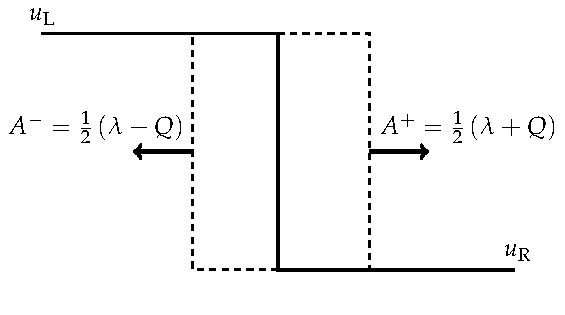
\includegraphics[width=0.47\textwidth,height=0.25\textwidth]
	{Figures/Theory/ScalarWaves-figure0.eps}}	
	\hspace{0.05\textwidth}
	\subfloat[Wave formulation]
	{\label{fig:waves}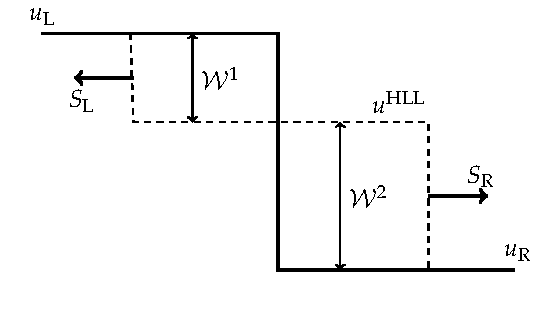
\includegraphics[width=0.47\textwidth,height=0.25\textwidth]
	{Figures/Theory/ScalarWaves-figure1.eps}}
	
	\captionsetup{justification=centering}
	
	\caption{Geometrical interpretation of how different numerical forms split the discontinuity.}
	\label{fig:FDS-waves}
\end{figure} 

Since the HLL-type scheme consists of two waves, we can write the updating formula for $ u_j^{n+1} $ in the wave propagation form (see~\cite[p.~80]{lev01}):
\begin{equation} \label{eq:scalar-W}
u_j^{n+1} = u_j - \frac{\Delta t}{\Delta x} \left( \sum_{p=1}^{2} S_{j-1/2}^{p,+} \mathcal{W}_{j-1/2}^p + \sum_{p=1}^{2} S_{j+1/2}^{p,-} \mathcal{W}_{j+1/2}^p \right), 
\end{equation}
where we introduce the notation $ S^{p,+} = \max \left( 0, S^p \right) $, $ S^{p,-} = \min \left( 0, S^p \right) $, and we define the wave velocities:
\begin{equation} \label{eq:scalar-W-S}
S_{j+1/2}^1 = \SLj, \quad S_{j+1/2}^2 = \SRj,
\end{equation}
and the waves:
\begin{equation} 
\mathcal{W}_{j+1/2}^1 = u_{j+1/2}^\text{HLL} - u_{j}, \quad \mathcal{W}_{j+1/2}^2 = u_{j+1} - u_{j+1/2}^\text{HLL}.
\end{equation}
For standard, one-parameter methods it is easy to show that:
\begin{align}
\ASj^- \Delta u_{j+1/2}
= & \frac{1}{2} \left( \lambda_{j+1/2} - \QSj \right) \Delta u_{j+1/2} \notag \\
= & \SLj \left( u_{j+1/2}^\text{HLL} - u_j \right) =
\sum_{p=1}^{2} S_{j+1/2}^{p,-} \mathcal{W}_{j+1/2}^p, \\
\ASj^+ \Delta u_{j+1/2}
= & \frac{1}{2} \left( \lambda_{j+1/2} + \QSj \right) \Delta u_{j+1/2} \notag \\
= & \SRj \left( u_{j+1} - u_{j+1/2}^\text{HLL} \right) =
\sum_{p=1}^{2} S_{j+1/2}^{p,+} \mathcal{W}_{j+1/2}^p.
\end{align}
This new framework provides a new insight into some properties of one-parameter methods. For standard-one parameter methods, \eqref{eq:scalar-W} becomes:
\begin{equation} \label{eq:scalar-W-oneQ}
u_j^{n+1} = u_j - \frac{\Delta t}{\Delta x} 
\left( 
Q_{\text{S},j-1/2} \left( u_{j} - u_{j-1/2}^\text{HLL} \right) - 
Q_{\text{S},j+1/2} \left( u_{j+1/2}^\text{HLL} - u_j \right) 
\right), 
\end{equation}
where by using \eqref{eq:HLL-NV-Qs} in \eqref{eq:scalar-uHLL} we have that an intermediate state of a one-parameter method is:
\begin{equation} \label{eq:scalar-uHLL1}
u_{j+1/2}^\text{HLL(1)} = \frac{1}{2} \left( u_{j} + u_{j+1} \right) - \frac{1}{2} \frac{\lambda_{j+1/2}}{\QSj}\left( u_{j+1} - u_j \right).
\end{equation}
By looking at \cref{fig:FDS-waves} we heuristically argue that the intermediate state of the one-parameter method should lie between the left and right state:
\begin{equation} \label{eq:scalar-waves-TVD}
u_{j+1/2}^\text{HLL(1)} \, \in \, \left[ \min \left( u_j, u_{j+1} \right), \max \left( u_j, u_{j+1} \right) \right].
\end{equation}
By enforcing this condition we find it is satisfied for:
\begin{equation} \label{eq:scalar-waves-lowerTVD}
\left| \lambda_{j+1/2} \right| \leq \QSj, \quad \forall \, j,
\end{equation}
which we recognize as the lower bound of the TVD condition \eqref{eq:3-NV-TVD}. We can see that in the wave propagation form, the upper bound of TVD condition limits how far can waves travel, while the lower bound limits the magnitude of the waves. We can show that \eqref{eq:scalar-waves-lowerTVD} implies \eqref{eq:scalar-waves-TVD} by rewriting \eqref{eq:scalar-waves-TVD} as:
\begin{align} 
u_j \geq u_{j+1/2}^\text{HLL(1)} \geq u_{j+1} \quad & \text{if} \quad u_{j} \geq u_{j+1}, \\
u_j \leq u_{j+1/2}^\text{HLL(1)} \leq u_{j+1} \quad & \text{if} \quad u_{j} \leq u_{j+1}.
\end{align}
We suppress the interface indices and observe that when $ u_{j} \geq u_{j+1} $, the left inequality can be rewritten as:
\begin{equation}
\frac{1}{2} \left( 1- \frac{\lambda}{Q_\text{S}} \right) \left( u_{j+1} - u_j \right) \leq 0.
\end{equation}
Since $ u_{j+1} - u_j \leq 0 $, we require that:
\begin{equation}
1 - \frac{\lambda}{Q_\text{S}} \geq 0.
\end{equation}
For $ \lambda > 0 $, we obtain that:
\begin{equation}
Q_\text{S} \geq |\lambda|,
\end{equation}
while for $ \lambda < 0 $ we obtain:
\begin{equation}
1 + \frac{|\lambda|}{Q_\text{S}} \geq 0,
\end{equation}
which is satisfied for any $ Q_\text{S} \geq 0 $. The remaining cases are done in the same way.

We can make several observation by considering $ u_{j+1/2}^\text{HLL(1)} $, eq. \eqref{eq:scalar-uHLL1}. The Roe scheme in flux-difference splitting form consists of a single discontinuity traveling either to the left or right, i.e. either $ A_\text{Roe}^{-} = 0 $ or $ A_\text{Roe}^{+} = 0 $. The wave propagation form consists of two waves traveling to the left and right, but it can be shown that by using $ Q_\text{Roe} $ in \eqref{eq:scalar-uHLL1} we obtain that either $ u_{j+1/2}^\text{HLL} = u_j $ or $ u_{j+1/2}^\text{HLL} = u_{j+1} $, hence one of the waves $ \mathcal{W} $ is equal to zero. This fits into the discussion above, since the Roe scheme is precisely the lower limit of the TVD condition.

Next, for the Lax-Wendroff scheme, $ Q_\text{L-W} = \lambda^2 \Delta t / \Delta x $, we obtain:
\begin{equation} 
u_{j+1/2}^\text{HLL-LW} = \frac{1}{2} \left( u_{j} + u_{j+1} \right) - \frac{1}{2} \frac{1}{\lambda} \frac{\Delta x}{\Delta t} \left( u_{j+1} - u_j \right),
\end{equation}
and the intermediate state is outside $ \mathcal{R} $, except when $ |\lambda|=\Delta x / \Delta t $.\footnote{Second-order accurate schemes are often achieved by using the \textit{wave limiters} which, as the name suggests, limit the magnitude of the waves $ \mathcal{W} $. Author conjectures that TVD wave limiters are precisely those that ensure that, at the discontinuities, the intermediate state lies within $ \mathcal{R} $.}

Further, in the case of transonic shock or transonic rarefaction when $ \lambda = 0 $, the Roe and Lax-Wendroff schemes do not have well defined intermediate state, since term $ \lambda/Q_\text{S} $ in \eqref{eq:scalar-uHLL1} becomes $ 0/0 $ and $ \Delta x /0 $, respectively.

Finally, we know that for the central scheme $ Q_\text{C} = 0 $. By using this in \eqref{eq:scalar-uHLL} the fraction on the right-hand side explodes, which explains why the scheme is unstable.

\subsection{Convergence and entropy stability}

We are now interested in convergence and entropy stability of the HLL-type scheme. As in previous chapter, we start by considering convergence to a weak solution along the lines of the Lax-Wendroff theorem. Then, we obtain stronger conditions to ensure convergence to the entropy solution.

\subsubsection*{Convergence}
The question of conservation was already discussed and we do not repeat it here. Consistency may be shown as earlier, by using the modified equation:
\begin{lemma}[Prebeg~\cite{cp2}] \label{lemma:HLL-consistent}
The HLL scheme with the numerical viscosity coefficient \eqref{eq:scalar-Q-HLL} is consistent with the scalar conservation law:
\begin{equation} \label{eq:SCL3}
u_t + f(u)_x = 0.
\end{equation}
\end{lemma}

\begin{proof}
Standard first-order methods give a second-order accurate approximation to the equation:
\begin{equation} \label{eq:3-ME3}
u_t + f(u)_x = \frac{1}{2} \frac{\Delta x^2}{\Delta t}\left[ \left( \frac{\Delta t}{\Delta x} \bar{Q} - c^2 \right) u_x \right]_x.
\end{equation}
By using \eqref{eq:scalar-Q-HLL} in \eqref{eq:3-ME3} we obtain that the HLL scheme gives a second-order accurate approximation to the equation:
\begin{equation} \label{eq:3-ME-HLL}
u_t + f(u)_x = \frac{1}{2} \frac{\Delta x^2}{\Delta t} \left[ D_{\text{HLL}} u_x \right]_x,
\end{equation}
where:
\begin{align}
D_{\text{HLL}} & = \frac{c - \CL}{\CR - \CL} \left( |\CR| - \CR^2 \right) \notag \\
& + \frac{\CR - c}{\CR - \CL} \left( |\CL|- \CL^2 \right) + \left( c - \CL \right) \left( \CR - c \right),
\end{align}
where $ \CL = \SL \Delta t / \Delta x $ and $ \CR = \SR \Delta t / \Delta x $. By keeping $ c = \text{const.} $ and passing $ \Delta x \rightarrow 0 $ we recover the scalar conservation law \eqref{eq:SCL3}.
\end{proof}

Next, we obtain conditions for the TVD stability:
\begin{lemma} \label{lemma:HLL-TVD}
The HLL scheme with the numerical viscosity coefficient \eqref{eq:scalar-Q-HLL} is TVD if:
\begin{equation} \label{eq:TVD-HLL-condition}
- \frac{\Delta x}{\Delta t} \leq
\SLj \leq 
\lambda_{j+1/2} \leq 
\SRj \leq
\frac{\Delta x}{\Delta t},
\quad \forall \, j.
\end{equation}
\end{lemma}

\begin{proof}
We suppress the interface indices and recall that a standard conservative scheme is unconditionally TVD if and only if:
\begin{equation}
\left| \lambda \right| \leq Q \leq \frac{\Delta x}{\Delta t},
\end{equation}
where for $ Q_{\text{HLL}} $ we require the following:
\begin{equation} \label{eq:TVD-HLL}
\left| \lambda \right| \leq \frac{\left| \SR \right| \left( \lambda - \SL \right) + \left| \SL \right| \left( \SR - \lambda \right)}{\SR - \SL} \leq \frac{\Delta x}{\Delta t}.
\end{equation}
The upper bound in \eqref{eq:TVD-HLL} can be rewritten as:
\begin{equation}
\left( \lambda - \SL \right) \left( |\SR|- \frac{\Delta x}{\Delta t} \right) + \left( \SR-\lambda \right) \left( |\SL|-\frac{\Delta x}{\Delta t} \right) \leq 0,
\end{equation}
which is always satisfied when the outer inequalities in \eqref{eq:TVD-HLL-condition} hold. The lower bound in \eqref{eq:TVD-HLL} can be rewritten as:
\begin{equation} 
\left( \lambda - \SL \right) \left( |\SR|- |\lambda| \right) + \left( \SR-\lambda \right) \left( |\SL|- |\lambda| \right) \geq 0, \label{eq:TVD-HLL-lower}
\end{equation}
which is always satisfied when the inner inequalities in \eqref{eq:TVD-HLL-condition} hold. \end{proof}

%We have the following result:
%\begin{proposition}
%The HLL scheme with the choice of wave velocities:
%\begin{equation} \label{eq:TVD-HLL-condition2}
%- \frac{\Delta x}{\Delta t} \leq
%\SLj \leq 
%\lambda_{j+1/2} \leq 
%\SRj \leq
%\frac{\Delta x}{\Delta t},
%\quad \forall \, j,
%\end{equation}
%converges to a weak solution of the scalar conservation law \eqref{eq:SCL2}.
%\end{proposition}
%
%\begin{proof}
%This follows from the Lax-Wendroff theorem, since the HLL scheme is conservative, consistent~(\Cref{lemma:HLL-consistent}) and TVD under the condition \eqref{eq:TVD-HLL-condition2}~(\Cref{lemma:HLL-TVD}).
%\end{proof}

\subsubsection*{Entropy stability}

%The convergence result above does not tell us if the scheme converges to the unique weak solution of the scalar conservation law. We can show that a scheme is entropy stable by using entropy functions, by showing that it is an E-scheme or by showing that it is monotone.

The TVD stability result above does not tell us if the scheme converges to the unique entropy-satisfying weak solution of the scalar conservation law. We can show that a scheme is entropy stable by using entropy functions, by showing that it is an E-scheme or by showing that it is monotone.

Herein, we will use entropy functions to show that the HLL scheme with the choice of the wave velocities according to Einfeldt~\cite{ein88}:
\begin{subequations} \label{eq:scalar-Einfeldt}
\begin{align}
\SL & = \min \left( \lambda_{j+1/2}, f'(u_j) \right), \\
\SR & = \max \left( \lambda_{j+1/2}, f'(u_{j+1}) \right),
\end{align}
\end{subequations}
is entropy stable.\footnote{In Einfeldt's paper~\cite{ein88}, the HLLE scheme is developed for the Euler equations. We will denote the choice \eqref{eq:scalar-Einfeldt} as the scalar HLLE because it is equivalent to applying the original Einfeldt's choice to the scalar conservation law.} Our proof closely follows the proof by Pelanti et al.~\cite[p.~12]{pel01} (see also~\cite{har83c,god96}).

We consider the discrete Riemann problem \eqref{eq:scalar-RP} for the scalar conservation law \eqref{eq:SCL2} with a convex flux function $ f(u) $. If the solution to the Riemann problem is supposed to be a shock \eqref{eq:scalar-shock}, the HLLE scheme yields $ \SL = \SR = \lambda $, and it can be shown that in the limit when $ \SL, \SR \rightarrow \lambda $, the HLLE scheme becomes the Roe scheme and the solution is:
\begin{equation} 
\widetilde{u}(x/t) = \left\{ \begin{array}{lll}
	u_\text{L} \quad & \text{if} \quad x < \lambda t, \\[0.25em]
	u_\text{R}		 & \text{if} \quad x > \lambda t. \end{array} \right.
\end{equation}
If the solution is supposed to be a rarefaction \eqref{eq:scalar-rarefaction}, the HLLE scheme yields $ \SL = f'(u_j) $ and $ \SR = f'(u_{j+1}) $, and the solution is:
\begin{equation} \label{eq:scalar-HLLE-r}
\widetilde{u}(x/t) = \left\{ \begin{array}{lll}
	u_\text{L}\quad & \text{if} \quad x < f'(u_\text{L}) t, \\[0.25em]
	u^\text{HLL}	& \text{if} \quad f'(u_\text{L}) t < x < f'(u_\text{R}) t, \\[0.25em]
	u_\text{R}      & \text{if} \quad x > f'(u_\text{R}) t. \end{array} \right.
\end{equation}
If the rarefaction is a \textit{transonic} rarefaction, i.e. \mbox{$ f'(u_\text{L}) < 0 <f'(u_\text{R}) $}, certain schemes (such as the Roe scheme) may lead to an entropy violation. If the HLLE scheme is entropy stable, the solution \eqref{eq:scalar-HLLE-r} must satisfy the integral form of the entropy condition \eqref{eq:SCL-entropy-inequality}:
\begin{equation} \label{eq:integral-EC}
\int_{0}^{\Delta t} \int_{-\frac{\Delta x}{2}}^{\frac{\Delta x}{2}} \left[ \eta (u)_t + \psi(u)_x \right] \diff x \diff t \leq 0.
\end{equation}
By using $ u = \widetilde{u}(x/t) $ and integrating \eqref{eq:integral-EC} we obtain:
\begin{equation}
\int_{-\frac{\Delta x}{2}}^{\frac{\Delta x}{2}} \eta (\widetilde{u}(x/\Delta t)) \diff x \leq 
\frac{\Delta x}{2} \left( \eta (u_\text{L}) + \eta (u_\text{R}) \right) - 
\Delta t \left( \psi(u_\text{R}) - \psi (u_\text{L}) \right).
\end{equation}
Since \eqref{eq:scalar-HLLE-r} consists of piecewise constant data, the left-hand side is:
\begin{align} \label{eq:HLLE-expanded}
\int_{-\frac{\Delta x}{2}}^{\frac{\Delta x}{2}} \eta (\widetilde{u}(x/ \Delta t)) \diff x
& = 
\eta(u^\text{HLL}) \left( \SR \Delta t - \SL \Delta t \right) \notag \\
& + \eta(u_\text{L}) \left( \SL \Delta t + \frac{\Delta x}{2} \right)
  + \eta(u_\text{R}) \left( \frac{\Delta x}{2} - \SR \Delta t \right). 
\end{align}
The outer bounds enclosing $ u^\text{HLL} $ in \eqref{eq:scalar-HLLE-r} are physical signal velocities that also appear in the exact solution \eqref{eq:scalar-rarefaction}, so we know from the conservation principle that $ u^\text{HLL} $ is equal to the integral of the exact solution $ u^\text{E}(x/t) $ from $ f'(u_\text{L}) \Delta t $ to $ f'(u_\text{R}) \Delta t $:
\begin{equation}
u^\text{HLL} = \frac{1}{\Delta t \left( \SR - \SL \right)} \int_{\SL \Delta t}^{\SR \Delta t} u^E(x/\Delta t) \diff x,
\end{equation}
where we used that $ \SL = f'(u_\text{L}) $ and $ \SR = f'(u_\text{R}) $ are the outer bounds of the exact solution \eqref{eq:scalar-rarefaction}. By using Jensen's inequality we have that:
\begin{equation} \label{eq:HLLE-Jensen}
\eta(u^\text{HLL}) \leq \frac{1}{\Delta t \left( \SR - \SL \right)} \int_{\SL t}^{\SR t} \eta(u^\text{E}(x/\Delta t)) \diff x .
\end{equation}
By using \eqref{eq:HLLE-Jensen} in \eqref{eq:HLLE-expanded} we obtain:
\begin{align}
\int_{-\frac{\Delta x}{2}}^{\frac{\Delta x}{2}} \eta (\widetilde{u}(x/\Delta t)) \diff x
& \leq 
\int_{\SL \Delta t}^{\SR \Delta t} \eta(u^\text{E}(x/ \Delta t)) \diff x \notag \\
& + \eta(u_\text{L}) \left( \SL t + \frac{\Delta x}{2} \right)
  + \eta(u_\text{R}) \left( \frac{\Delta x}{2} - \SR \Delta t \right),
\end{align}
where the right-hand side is the exact solution:
\begin{align}
\int_{-\frac{\Delta x}{2}}^{\frac{\Delta x}{2}} \eta (\widetilde{u}(x/\Delta t)) \diff x
& \leq
\int_{-\frac{\Delta x}{2}}^{\frac{\Delta x}{2}} \eta (u^\text{E}(x/\Delta t)) \diff x \notag \\
& \leq \frac{\Delta x}{2} \left( \eta (u_\text{L})
     + \eta (u_\text{R}) \right) - \Delta t \left( \psi(u_\text{R}) - \psi (u_\text{L}) \right),
\end{align}
where the last inequality follows from the fact that the exact solution satisfies the entropy inequality. Hence, we showed that the HLLE scheme is entropy stable, provided that the TVD condition \eqref{eq:TVD-HLL-condition} is satisfied.

\subsection{LTS-HLL scheme for scalar conservation laws}

In addition to the numerical viscosity and the flux-difference splitting form, we recall that it was also possible to write the updating formula of a standard method in terms of the solutions to the neighboring Riemann problems (see \eqref{eq:convex-update}):
\begin{equation} \label{eq:convex-update2}
u_j^{n+1} =
\frac{1}{\Delta x}
\int_{0}^{\frac{\Delta x}{2}} \widetilde{u}_{j-1/2} \left( x/ \Delta t \right) \diff x +
\frac{1}{\Delta x}
\int_{-\frac{\Delta x}{2}}^{0} \widetilde{u}_{j+1/2} \left( x/ \Delta t \right) \diff x,
\end{equation}
where $ \widetilde{u}_{j-1/2}(x/t) $ is the approximate solution to the local Riemann problem at the cell interface $ x_{j-1/2} $. Since in LTS method the value of $ u_j^{n+1} $ may depend on more than three cells, it might also depend on more than two Riemann problems. Following LeVeque~\cite{lev85} (see also Lindqvist et al.~\cite{lin16}) we may write the general updating formula of LTS method in terms of solutions to all Riemann problems in the domain of dependence:
\begin{equation} \label{eq:scalar-LTS-update}
u_j^{n+1} = \frac{\Delta t}{\Delta x} \sum\limits_{i=-\infty}^{\infty} \int_{(i-1)\frac{\Delta x}{\Delta t}}^{i \frac{\Delta x}{\Delta t}} \widetilde{u}_{j+1/2-i} \diff \xi_i - \sum\limits_{l=-\infty}^{\infty} u_l,
\end{equation}
where $ \widetilde{u}_{j+1/2-i} $ is the solution to the Riemann problem at $ x_{j+1/2-i} $ and:
\begin{equation}
\xi_i = \frac{x - x_{j+1/2-i}}{t - t^n}.
\end{equation}
We note that \eqref{eq:scalar-LTS-update} reduces to \eqref{eq:convex-update2} when $ \bar{C} \leq 1 $.

To obtain the numerical viscosity and flux-difference splitting coefficients of the LTS-HLL scheme, we follow our paper~\cite{jp2} and use \eqref{eq:scalar-RP-HLL} in \eqref{eq:scalar-LTS-update} to determine the flux-difference splitting coefficients, and then use the formula \eqref{eq:FDS-NV} to directly obtain the numerical viscosity coefficients. For a slightly different approach, which includes geometrical consideration and more heuristic arguments we also refer to our paper~\cite{jp2}, where as the starting point we used HLL(C) schemes for systems of equations.

\begin{proposition}[Prebeg et al.~\cite{jp2}] \label{prop:LTS-HLL-A}
The LTS-HLL scheme can be written in the flux-difference splitting form \eqref{eq:scalar-LTS-FDS} with coefficients:
\begin{align} \label{eq:scalar-LTS-HLL-A}
A_\text{HLL}^{i\pm} = & \pm \frac{\lambda - \SL}{\SR - \SL} \max \left( 0, \min \left( \pm \SR - i \frac{\Delta x}{\Delta t}, \frac{\Delta x}{\Delta t} \right) \right) \notag \\
& \pm \frac{\SR - \lambda}{\SR - \SL} \max \left( 0, \min \left( \pm \SL - i \frac{\Delta x}{\Delta t}, \frac{\Delta x}{\Delta t} \right) \right). 
\end{align}
\end{proposition}

\begin{proof}
The HLL Riemann solver \eqref{eq:scalar-RP-HLL} can be written as:
\begin{subequations}
\begin{align}
\widetilde{u}_{j+1/2}(\zeta) & = u_j + H(\zeta - \SL) \left( u_{j+1/2}^\text{HLL} - u_j \right) + H( \zeta - \SR) \left( u_{j+1} - u_{j+1/2}^\text{HLL} \right) \\
&=u_{j+1}-H(\SL-\zeta)\left(u_{j+1/2}^\text{HLL}-u_j\right)-H(\SR-\zeta)\left(u_{j+1}-u_{j+1/2}^\text{HLL}\right),
\end{align}
\end{subequations}
where $H$ is the Heaviside function. By using \eqref{eq:scalar-uHLL} we can rewrite this as:
\begin{subequations}
\begin{align}
\widetilde{u}_{j+1/2}(\zeta) 
& = 
u_j +
\left( \frac{H(\zeta-\SL)}{\SR-\SL}(\SR-\lambda) +
\frac{H(\zeta-\SR)}{\SR-\SL}(\lambda-\SL)
\right) (u_{j+1}-u_j) \label{eq:uzeta-a} \\
& = u_{j+1} -
\left( \frac{H(\SL-\zeta)}{\SR-\SL}(\SR-\lambda) +
\frac{H(\SR-\zeta)}{\SR-\SL}(\lambda-\SL)
\right)(u_{j+1}-u_j). \label{eq:uzeta-b}
\end{align}
\end{subequations}
We then use \eqref{eq:uzeta-a} in \eqref{eq:scalar-LTS-update} and note that for $i\leq 0$ we can write:
\begin{equation}\label{eq:negi}
\int_{(i-1)\frac{\Delta x}{\Delta t}}^{i\frac{\Delta x}{\Delta t}} \widetilde{u}_{j+1/2-i} (\zeta_i) \diff \zeta_i = 
\frac{\Delta x}{\Delta t} u_{j-i}-A_{j+1/2-i}^{(-i)-}\left(u_{j+1-i}-u_{j-i}\right),
\end{equation}
where $ A^{i-} $ is the flux-difference splitting coefficient:
\begin{align}\label{eq:scalar-HLL-Aminus}
A_\text{HLL}^{i-} & = \frac{\lambda - \SL}{\SR - \SL} \min \left( 0, \max \left( \SR + i \frac{\Delta x}{\Delta t}, -\frac{\Delta x}{\Delta t} \right) \right) \notag \\
& + \frac{\SR - \lambda}{\SR - \SL} \min \left( 0, \max \left( \SL + i \frac{\Delta x}{\Delta t}, -\frac{\Delta x}{\Delta t} \right) \right). 
\end{align}
Similarly, we use \eqref{eq:uzeta-b} in \eqref{eq:scalar-LTS-update} and note that for $i\geq 1$ we can write:
\begin{equation}\label{eq:posi}
\int_{(i-1)\frac{\Delta x}{\Delta t}}^{i\frac{\Delta x}{\Delta t}} \widetilde{u}_{j+1/2-i} (\zeta_i)\diff \zeta_i=\frac{\Delta x}{\Delta t}u_{j+1-i}- A_{j+1/2-i}^{(i-1)+}\left(u_{j+1-i}-u_{j-i}\right),
\end{equation}
where $ A^{i+} $ is the flux-difference splitting coefficient:
\begin{align}\label{eq:scalar-HLL-Aplus}
A_\text{HLL}^{i+} & = \frac{\lambda - \SL}{\SR - \SL} 
\max \left( 0, \min \left( \SR - i \frac{\Delta x}{\Delta t}, \frac{\Delta x}{\Delta t} \right) \right) \notag \\
& + \frac{\SR - \lambda}{\SR - \SL} 
\max \left( 0, \min \left( \SL - i \frac{\Delta x}{\Delta t}, \frac{\Delta x}{\Delta t} \right) \right). 
\end{align}
Substituting \eqref{eq:negi} and \eqref{eq:posi} into \eqref{eq:scalar-LTS-update} we recover the LTS method in the flux-difference splitting form \eqref{eq:scalar-LTS-FDS}.
\end{proof}

\begin{proposition}[Prebeg et al.~\cite{jp2}]
The LTS-HLL scheme can be written in the numerical viscosity form \eqref{eq:scalar-LTS-NV} with coefficients:
\begin{subequations} \label{eq:scalar-LTS-HLL-Q}
\begin{align}
Q_\text{HLL}^0 & = \frac{\left| \SR \right| \left( \lambda - \SL \right) + \left| \SL \right| \left( \SR - \lambda \right) }{\SR - \SL}, \\
Q_\text{HLL}^{\mp i} & = 2 \frac{\lambda - \SL}{\SR - \SL} \max \left( 0, \pm \SR - i \frac{\Delta x}{\Delta t} \right) \notag \\
& + 2 \frac{\SR - \lambda}{\SR - \SL} \max \left( 0, \pm \SL - i \frac{\Delta x}{\Delta t} \right) \quad \text{for} \quad i>0. 
\end{align} 
\end{subequations}
\end{proposition}

\begin{proof}
Use \eqref{eq:scalar-LTS-HLL-A} in \eqref{eq:FDS-NV} to recover \eqref{eq:scalar-LTS-HLL-Q}.
\end{proof}

In addition to NV and FDS form, we may also write the LTS-HLL scheme in the wave propagation form \eqref{eq:scalar-W}:
\begin{equation} \label{eq:scalar-LTS-W}
u_j^{n+1} = u_j - \frac{\Delta t}{\Delta x} \sum\limits_{i=0}^{\infty} \left( \sum\limits_{p=1}^{2} S_{j-1/2-i}^{p,i+} \mathcal{W}_{j-1/2-i}^p + \sum\limits_{p=1}^{2} S_{j+1/2+i}^{p,i-} \mathcal{W}_{j+1/2+i}^p \right),
\end{equation}
where we recall that $ S^1 = \SL $ and $ S^2 = \SR $ (eq. \eqref{eq:scalar-W-S}). The wave velocities \eqref{eq:scalar-W-S} are modified as:
\begin{equation} \label{eq:scalar-LTS-W-S}
S^{p,i\pm} = \pm \max \left( 0, \min \left( \pm S^p - i \frac{\Delta x}{\Delta t}, \frac{\Delta x}{\Delta t} \right) \right).
\end{equation}
We recall that the interface indices on $ A $, $ Q $ and $ S^p $ have been suppressed, and we refer to \cref{rem:indexing} (p.~\pageref{eq:scalar-LTS-Roe-NV}) for explanation of the notation.

\subsection{A class of LTS one-parameter methods}
\label{cha3:sec:LTS-one-parameter}

In \Cref{prop:HLL-NV-Qs,prop:HLL-FDS-As} we showed that the standard one-parameter methods \eqref{eq:scalar-Q} and \eqref{eq:scalar-A} can be deduced from the HLL-type scheme by appropriate choice of $ \SL $ and $ \SR $. This motivated the question if we can obtain LTS one-parameter methods from the the LTS-HLL-type scheme by appropriate choice of $ \SL $ and $ \SR $. 

We begin with the LTS-Roe and LTS-Lax-Friedrichs schemes because we already have their NV and FDS coefficients. We may recover the LTS-Roe scheme in the NV \eqref{eq:scalar-LTS-Roe-NV} and FDS \eqref{eq:scalar-LTS-Roe-FDS} form by using:
\begin{equation}
\SL = - Q_\text{Roe}, \quad \SR = Q_\text{Roe},
\end{equation}
in the LTS-HLL-type scheme in the NV \eqref{eq:scalar-LTS-HLL-Q} and FDS \eqref{eq:scalar-LTS-HLL-A} form, respectively. In order to obtain the LTS-Lax-Friedrichs scheme in the NV \eqref{eq:scalar-LTS-LxF-NV} and FDS \eqref{eq:scalar-LTS-LxF-FDS} form, we must use:
\begin{equation}
\SL = - k Q_\text{LxF}, \quad \SR = k Q_\text{LxF},
\end{equation}
in the LTS-HLL-type scheme in the NV \eqref{eq:scalar-LTS-HLL-Q} and FDS \eqref{eq:scalar-LTS-HLL-A} form, respectively. This illuminates an important point related to the Lax-Friedrichs scheme. The numerical viscosity coefficient of the standard Lax-Friedrichs scheme \eqref{eq:scalar-Q-LxF} was defined as:
\begin{equation} \label{eq:scalar-Q-LxF1}
Q_\text{LxF} = \Delta x / \Delta t,
\end{equation}
while the partial numerical viscosity coefficient of the LTS-Lax-Friedrichs scheme \eqref{eq:scalar-LTS-LxF-NV} associated with $ i=0 $ was defined as:
\begin{equation} \label{eq:scalar-LTS-LxF-Q0}
Q_\text{LTS-LxF}^0 = k \Delta x / \Delta t.
\end{equation}
In order to obtain the LTS-Lax-Friedrichs scheme \eqref{eq:scalar-LTS-LxF-NV} from the LTS-HLL-type scheme \eqref{eq:scalar-LTS-HLL-Q}, we must use \eqref{eq:scalar-LTS-LxF-Q0}. We can now see that in the standard Lax-Friedrichs scheme \eqref{eq:scalar-Q-LxF1} the coefficient $ k=1 $ is implicitly assumed, and that the numerical viscosity coefficient of the standard method in fact reads $ Q_\text{LxF} = k \Delta x / \Delta t $.

Having obtained the LTS-Roe and LTS-Lax-Friedrichs schemes by following the approach used for standard methods (see \Cref{prop:HLL-NV-Qs,prop:HLL-FDS-As}), we establish equivalent results for other LTS methods.

\begin{proposition}\label{prop:LTS-HLL-NV-Qs}
Consider a first-order accurate, LTS one-parameter conservative scheme written in the numerical viscosity form \eqref{eq:scalar-LTS-NV}, which is uniquely determined by the partial numerical viscosity coefficients $ Q_\text{S}^i $. By defining $ \SL $ and $ \SR $ in the LTS-HLL-type scheme \eqref{eq:scalar-LTS-HLL-Q} as:
\begin{equation} \label{eq:LTS-HLL-NV-Qs}
\SL = -Q_\text{S}, \quad \SR = Q_\text{S},
\end{equation}
the numerical viscosity coefficients of the HLL-type scheme become:
\begin{subequations} \label{eq:scalar-LTS-NV-oneQ}
\begin{align}
Q_\text{HLL}^0 & = Q_\text{S}, \\
Q_\text{HLL}^{\mp i} & = \frac{\lambda - Q_\text{S}}{Q_\text{S}} \max \left( 0, \pm Q_\text{S} - i \frac{\Delta x}{\Delta t} \right) \notag \\
& +\frac{Q_\text{S} - \lambda}{Q_\text{S}} \max \left( 0, \mp Q_\text{S} - i \frac{\Delta x}{\Delta t} \right) \quad \text{for}\quad i>0. 
\end{align} 
\end{subequations}
\end{proposition}

\begin{proof}
Use \eqref{eq:LTS-HLL-NV-Qs} in \eqref{eq:scalar-LTS-HLL-Q} to obtain \eqref{eq:scalar-LTS-NV-oneQ}.
\end{proof}

\begin{proposition}\label{prop:LTS-HLL-FDS-As}
Consider a first-order accurate, LTS one-parameter conservative scheme written in the flux-difference splitting form \eqref{eq:scalar-LTS-FDS}, which is uniquely determined by the flux-difference splitting coefficients $ A_\text{S}^{i\pm} $. By defining $ \SL $ and $ \SR $ in the LTS-HLL-type scheme \eqref{eq:scalar-LTS-HLL-Q} as:
\begin{equation} \label{eq:LTS-HLL-FDS-As}
\SL = A_\text{S}^- - A_\text{S}^+ = - Q_\text{S}, \quad \SR = A_\text{S}^+ - A_\text{S}^- = Q_\text{S},
\end{equation}
the flux-difference splitting coefficients of the HLL-type scheme become:
\begin{align} \label{eq:scalar-LTS-FDS-oneA}
A_\text{S}^{i\pm} = & \pm \frac{\lambda + Q_\text{S}}{2 Q_\text{S}} \max \left( 0, \min \left( \pm Q_\text{S} - i \frac{\Delta x}{\Delta t}, \frac{\Delta x}{\Delta t} \right) \right) \notag \\
& \pm \frac{Q_\text{S} - \lambda}{2 Q_\text{S}} \max \left( 0, \min \left( \mp Q_\text{S} - i \frac{\Delta x}{\Delta t}, \frac{\Delta x}{\Delta t} \right) \right). 
\end{align}
\end{proposition}

\begin{proof}
Use \eqref{eq:LTS-HLL-FDS-As} is \eqref{eq:scalar-LTS-HLL-A} to obtain \eqref{eq:scalar-LTS-FDS-oneA}.
\end{proof}

We obtained a framework of LTS two-parameter methods that contains already existing LTS-Roe and LTS-Lax-Friedrichs schemes, and allows us to directly obtain an LTS extension of any first-order accurate standard one-parameter method. We note that an LTS extension of standard method is not unique. In our framework, what makes an LTS method an extension of a standard method is the fact that they are based on the same NV (or FDS) coefficients, and that the LTS method reduces to the standard method for $ \bar{C} \leq 1 $. Newly developed LTS extensions include:
\begin{itemize} \label{eq:LTS-1p-itemize}
\item \textit{LTS-Engquist-Osher:} Framework established above provides an LTS extension of the Engquist-Osher scheme. In the next section, we will show that our LTS-Engquist-Osher scheme is not entropy stable. On the other hand, Brenier~\cite{bre84} developed a monotone (hence entropy stable) LTS-Engquist-Osher scheme. Unfortunately, we do not know NV or FDS coefficients of the LTS-Engquist-Osher scheme by Brenier so at the moment we cannot compare these two.

\item \textit{LTS-Godunov:} Using $ \SL=-Q_\text{God} $ and $ \SR=Q_\text{God} $ does not recover the LTS-Godunov scheme of Lindqvist et al.~\cite{lin16}. In our framework, every scheme can be interpreted as the two-wave Riemann solver~\eqref{eq:scalar-RP-HLL}, and that also applies to our LTS-Godunov scheme when the solution is supposed to be a rarefaction. On the other hand, the LTS-Godunov scheme of Lindqvist et al.~\cite{lin16} splits a rarefaction into as many waves necessary to resolve it exactly (to projection error) on the given grid.

\item \textit{LTS-Lax-Wendroff:} \Cref{prop:LTS-HLL-NV-Qs,prop:LTS-HLL-FDS-As} are stated for first-order accurate schemes. A straightforward LTS extension of the Lax-Wendroff scheme seems to be unstable. This issue is currently being investigated, and as a possible cause of failure we note that for standard methods we have:
\begin{equation}
c^2 \leq |c| \leq 1 \quad \rightarrow \quad Q_\text{L-W} \leq Q_\text{Roe} \leq Q_\text{LxF}.
\end{equation}
However, for LTS methods with an arbitrary Courant number, the numerical viscosity coefficient of the Lax-Wendroff scheme may exceed both $ Q_\text{Roe} $ and $ Q_\text{LxF} $.
\end{itemize}

\subsection{Convergence and entropy stability}
\label{sec:LTS-HLL:C-ES-scalar-LTS}

\subsubsection*{Convergence} 

All considerations regarding the convergence of existing LTS methods (see section~\ref{sec:Background:C-ES-scalar-LTS}) also apply to LTS-HLL-type schemes. Namely, following the Lax-Wendroff theorem we are able to show that LTS-HLL-type methods with certain restrictions on the wave velocity estimates $ \SL $ and $ \SR $ converge to a weak solution.

The question of conservation was already discussed and we do not repeat it here. Consistency may be shown as earlier, by using the modified equation:
\begin{lemma}[Prebeg~\cite{cp2}] \label{lemma:LTS-HLL-consistent}
The LTS-HLL scheme with the numerical viscosity coefficient \eqref{eq:scalar-LTS-HLL-Q} is consistent with the scalar conservation law:
\begin{equation} \label{eq:SCL4}
u_t + f(u)_x = 0.
\end{equation}
\end{lemma}

\begin{proof}
First-order methods give a second-order accurate approximation to the equation:
\begin{equation} \label{eq:LTS-ME3}
u_t + f(u)_x = \frac{1}{2} \frac{\Delta x^2}{\Delta t} \left[ \left( \sum\limits_{i=1-k}^{k-1} \frac{\Delta t}{\Delta x} \bar{Q}^i - c^2 \right) u_x \right]_x.
\end{equation}
By using \eqref{eq:scalar-LTS-HLL-Q} in \eqref{eq:LTS-ME3} we obtain that the LTS-HLL scheme gives a second-order accurate approximation to the equation:
\begin{equation} \label{eq:LTS-ME-HLL}
u_t + f(u)_x = \frac{1}{2} \frac{\Delta x^2}{\Delta t} \left[ D_{\text{LTS-HLL}} u_x \right]_x,
\end{equation}
where:
\begin{align}
D_\text{LTS-HLL} & = \frac{c - \CL}{\CR - \CL} \left( \lceil |\CR| \rceil - |\CR| \right) \left( 1 + |\CR| - \lceil |\CR| \rceil \right) \notag \\ 
& + \frac{\CR - c}{\CR - \CL} \left( \lceil |\CL| \rceil - |\CL| \right) \left( 1 + |\CL| - \lceil |\CL| \rceil \right) \notag \\ 
& + \left( c - \CL \right) \left( \CR - c \right),
\end{align}
where $ \CL = \SL \Delta t / \Delta x $, $ \CR = \SR \Delta t / \Delta x $, and $ \lceil c \rceil = \min \{ n \in \mathbb{Z} \,| \, n \geq c \} $ is a ceiling function. By keeping $ c = \text{const.} $ and passing $ \Delta x \rightarrow 0 $ we recover the scalar conservation law \eqref{eq:SCL4}.
\end{proof}

To show TVD stability we use the TVD conditions for the LTS method in terms of the numerical viscosity coefficients, see \eqref{eq:LTS-TVD}.

\begin{lemma} \label{lemma:LTS-HLL-TVD}
The LTS-HLL scheme with the numerical viscosity coefficients \eqref{eq:scalar-LTS-HLL-Q} is TVD if:
\begin{equation} \label{eq:LTS-HLL-TVD}
\SLj \leq \lambda_{j+1/2} \leq \SRj, \quad \forall \, j.
\end{equation}
\end{lemma}

\begin{proof}
We suppress the interface indices and note that by substituting \eqref{eq:scalar-LTS-HLL-Q} in \eqref{eq:LTS-TVD-a}--\eqref{eq:LTS-TVD-c} the TVD conditions become:
\begin{subequations}
\begin{align}
  \left( \lambda - \SL \right) \left( \frac{\Delta x}{\Delta t} - \min \left( \left| \SR \right|, \frac{\Delta x}{\Delta t} \right) \right) & \notag \\ 
+ \left( \SR - \lambda \right) \left( \frac{\Delta x}{\Delta t} - \min \left( \left| \SL \right|, \frac{\Delta x}{\Delta t} \right) \right) 
& \geq 0, \\
  \left( \lambda - \SL \right) \max \left( 0, \min \left( \pm 2 \SR, 4 \frac{\Delta x}{\Delta t} \mp 2\SR \right) \right) \notag \\
+ \left( \SR - \lambda \right) \max \left( 0, \min \left( \pm 2 \SL, 4 \frac{\Delta x}{\Delta t} \mp 2\SL \right) \right)
& \geq 0, \\
  \left( \lambda - \SL \right) \max \left( 0, \min \left( \pm \SR - i \frac{\Delta x}{\Delta t}, \mp \SR + i \frac{\Delta x}{\Delta t} + 2 \right) \right) & \notag \\
+ \left( \SR - \lambda \right) \max \left( 0, \min \left( \pm \SL - i \frac{\Delta x}{\Delta t}, \mp \SL + i \frac{\Delta x}{\Delta t} + 2 \right) \right) & \geq 0 \quad \forall \quad i \geq 1,
\end{align}
\end{subequations}
which are always satisfied under the condition \eqref{eq:LTS-HLL-TVD}.
\end{proof}

%We have the following result:
%\begin{proposition}
%The LTS-HLL scheme with the choice of wave velocities:
%\begin{equation} \label{eq:TVD-LTS-HLL-condition}
%\SLj \leq \lambda_{j+1/2} \leq \SRj, \quad \forall \, j,
%\end{equation}
%converges to a weak solution of the scalar conservation law \eqref{eq:SCL4}.
%\end{proposition}
%
%\begin{proof}
%This follows from the Lax-Wendroff theorem, since the LTS-HLL scheme is conservative, consistent~(\Cref{lemma:LTS-HLL-consistent}) and TVD under the condition \eqref{eq:TVD-LTS-HLL-condition}~(\Cref{lemma:LTS-HLL-TVD}).
%\end{proof}

\subsubsection*{Entropy stability}

The discussion on entropy stability of existing LTS methods from \cref{sec:Background:C-ES-scalar-LTS} also applies here. We note that in general, the class of TVD LTS-HLL-type schemes is not entropy stable, because this class includes the entropy violating LTS-Roe scheme. We will address the question of entropy stability in LTS methods in \cref{sec:EV-ME} by using the modified equation analysis.

\subsection{LTS-HLL(C) schemes for systems of conservation laws}

The LTS-HLL-type schemes can be extended to systems of equations following the same way the already existing LTS methods have been extended to systems of equations, see~\cref{sec:Background:FVM-systems}. A slightly different approach to obtain the LTS-HLL scheme for systems of equations is given in our paper~\cite{jp2}, where we start with the standard HLL(C) schemes for systems of equations and extend them to the LTS framework. Our paper~\cite{jp2} also includes analysis of numerical diffusion in the LTS-HLL scheme for the Euler equations, and numerical results for both LTS-HLL(C) schemes applied to the Euler equations.

Up to now, we did not explicitly present the HLLC and the LTS-HLLC schemes. This is due to the fact that we did not develop a scalar counterpart of the HLLC scheme, and because the HLLC scheme does not naturally fit into the NV and FDS form. Nevertheless, an LTS-HLLC scheme in a conservation form can be obtained in a relatively straightforward manner and we refer to our papers~\cite{cp2,jp2} for more details.

Herein, we show that both LTS-HLL(C) schemes for systems of equations can be also written in the wave propagation form. This can be done by combining elements of wave propagation form and the HLLC scheme, as is done for instance by Pelanti and Shyue~\cite{pel14}. We skip technical details and give a final result.

An LTS scheme for scalar conservation law in the wave propagation form \eqref{eq:scalar-LTS-W} can be extended to systems of equations as:
\begin{equation} \label{eq:system-LTS-W}
\mathbf{U}_j^{n+1} = \mathbf{U}_j - 
\frac{\Delta t}{\Delta x} \sum\limits_{i=0}^{\infty} \left(
\sum\limits_{p=1}^{m} S_{j-1/2-i}^{p,i+} \mathcal{W}_{j-1/2-i}^p +
\sum\limits_{p=1}^{m} S_{j+1/2+i}^{p,i-} \mathcal{W}_{j+1/2+i}^p 
\right),
\end{equation}
where for the HLL scheme $ m=2 $, and the wave velocities are:
\begin{equation}
S^1 = S, \quad S^2 = \SR,
\end{equation}
while the waves are:
\begin{subequations}
\begin{align}
\mathcal{W}_{j-1/2}^1 & = \mathbf{U}_{j-1/2}^\text{HLL} - \mathbf{U}_{j-1}, \quad \\
\mathcal{W}_{j-1/2}^2 & = \mathbf{U}_{j} - \mathbf{U}_{j-1/2}^\text{HLL},
\end{align}
\end{subequations}
where $ \mathbf{U}_{j-1/2}^\text{HLL} $ is determined following the same principles as for the intermediate state in case of scalar conservation law \eqref{eq:scalar-uHLL}. For the HLLC scheme applied to one-dimensional Euler equations $ m=3 $, and the wave velocities are:
\begin{equation}
S^1 = \SL, \quad S^2 = S_\text{C}, \quad S^3 = \SR,
\end{equation}
while the waves are:
\begin{subequations}
\begin{align}
\mathcal{W}_{j-1/2}^1 & = \mathbf{U}_{\text{L},j-1/2}^\text{HLLC} - \mathbf{U}_{j-1}, \quad \\
\mathcal{W}_{j-1/2}^2 & = \mathbf{U}_{\text{R},j-1/2}^\text{HLLC} - \mathbf{U}_{\text{L},j-1/2}^\text{HLLC}, \quad \\
\mathcal{W}_{j-1/2}^3 & = \mathbf{U}_{j}^\text{HLLC} - \mathbf{U}_{\text{R},j-1/2}^\text{HLLC},
\end{align}
\end{subequations}
where the definition of the contact wave velocity $ S_\text{C} $ and the intermediate states $ \mathbf{U}_{\text{L,R},j-1/2}^\text{HLLC} $ can be found in our papers~\cite{cp2,jp2} and in paper by Toro et al.~\cite{tor94} and the book by Toro~\cite{tor09}, from where we adopted them. All velocities are modified in the same manner as:
\begin{equation} \label{eq:system-LTS-W-S}
S_\text{L,C,R}^{i\pm} = \pm \max \left( 0, \min \left( \pm S_\text{L,C,R} - i \frac{\Delta x}{\Delta t}, \frac{\Delta x}{\Delta t} \right) \right).
\end{equation}

\subsection{Choice of the wave velocity estimates $ \SL $ and $ \SR $}
\label{s:SLSR}

We now address the question on how to choose the wave velocity estimates $ \SL $ and $ \SR $. This question was left open in the original paper where the HLL scheme was introduced~\cite{har83a}, and was addressed by a number of authors in the coming years, see beginning of~\cref{sec:LTS-HLL(C)}. Herein, we outline some of velocity choices as applied to systems of equations, and we note that all of these also apply to the HLLC scheme and to the LTS extensions of the HLL(C) schemes.

We have already seen that for the scalar conservation laws, we can recover standard one-parameter methods from the standard HLL-type framework by an appropriate choice of $ \SL $ and $ \SR $. In addition, we constructed genuinely two-parameter HLLE scheme. For systems of conservation laws, we can exactly deduce one-parameter methods from the HLL-type framework only for systems with two equations. If system of equations has more than two equations, we can exactly deduce only those one-parameter methods which consist of two waves (such as the Lax-Friedrichs scheme), but not those schemes that consist of more than two waves (such as the Roe scheme). 

For example, by defining:
\begin{equation} \label{eq:system-SLSR-LxF}
\SLj = - k \Delta x / \Delta t, \qquad \SRj = k \Delta x / \Delta t,
\end{equation}
we obtain the eigenvalues $ (\omega^1,\dots,\omega^N) $ and $ (\lambda^1,\dots,\lambda^N) $ corresponding to the Lax-Friedrichs scheme, and by defining:
\begin{equation}
\SLj = -\SRj, \qquad
\SRj = \max ( |\lambda_j^1|,|\lambda_{j+1}^1|,|\lambda_j^N|,|\lambda_{j+1}^N| ),
\end{equation}
we obtain the eigenvalues $ (\omega^1,\dots,\omega^N) $ and $ (\lambda^1,\dots,\lambda^N) $ corresponding to the Rusanov scheme. We note that we will obtain genuine Lax-Friedrichs and Rusanov schemes independent of how many waves the system of equations has. By choosing:
\begin{equation} \label{eq:system-SLSR-Roe}
\SLj = \lambda_{\text{Roe},j+1/2}^1, \qquad
\SRj = \lambda_{\text{Roe},j+1/2}^N,
\end{equation}
we obtain the eigenvalues $ (\omega^1,\omega^N) $ and $ (\lambda^1,\lambda^N) $ corresponding to the Roe scheme. The choice \eqref{eq:system-SLSR-Roe} identically reduces to the Roe scheme only for systems with two waves. For standard methods, the above was observed already by Davis~\cite{dav88} and Einfeldt~\cite{ein88}.

Some other choices are given as:
\begin{equation} \label{eq:system-Davis1}
\left. \begin{array}{ll}
S_{\text{L},j+1/2} = \lambda_j^1 \\[0.5em]
S_{\text{R},j+1/2} = \lambda_{j+1}^N \end{array} \right. \qquad \text{Davis \#1~\cite{dav88}}.
\end{equation}
\begin{equation} \label{eq:system-Davis2}
\left. \begin{array}{ll}
S_{\text{L},j+1/2} = \min \left( \lambda_j^1,   \lambda_{j+1}^1 \right) \\[0.5em]
S_{\text{R},j+1/2} = \max \left( \lambda_{j}^N, \lambda_{j+1}^N \right) \end{array} \right. \qquad \text{Davis \#2~\cite{dav88}}.
\end{equation}
\begin{equation} \label{eq:system-Einfeldt}
\left. \begin{array}{ll}
S_{\text{L},j+1/2} = \min \left( \lambda_j^1, \lambda_{j+1/2}^1 \right) \\[0.5em]
S_{\text{R},j+1/2} = \max \left( \lambda_{j+1/2}^N, \lambda_{j+1}^N \right) \end{array} \right. \qquad \text{Einfeldt~\cite{ein88}}.
\end{equation} More complicated choices constructed for the Euler equations can be found in Toro et al.~\cite{tor94} and Bouchut~\cite{bou04}, where Bouchut developed a special choice of $ \SL $ and $ \SR $ in order to handle vacuum in the Euler equations. 

The choice of the wave velocities according to Einfeldt~\cite{ein88} is very popular among the standard methods, because it yields an entropy stable and a positivity preserving scheme~\cite{ein91}. Among the choices \eqref{eq:system-Davis1}--\eqref{eq:system-Einfeldt} and those found in Toro et al.~\cite{tor94}, Einfeldt's choice \eqref{eq:system-Einfeldt} was also found to yield the very best results when used in LTS-HLL(C) schemes. These observations are based on our experience, and more rigorous comparison may be fruitful.

The LTS-HLLE scheme for systems of equations seems to inherit the HLLE scheme property of being entropy stable, but does not inherit the HLLE scheme property of being positivity preserving. The former will be addressed in the next~\cref{sec:EV-ME}~\textit{Entropy stability} and it is a topic of our conference paper~\cite{cp2}, while the latter will be addressed in~\cref{sec:PP}~\textit{Positivity preservation} and it is a topic of our journal paper~\cite{jp3}. 
